\documentclass{beamer}
\usepackage[polish]{babel}
\usepackage[utf8]{inputenc}
\usepackage[T1]{fontenc}
\usepackage{svg}
\usepackage{animate}
\usepackage{graphicx}
\usepackage{svg}
\usepackage{xcolor}
\usepackage{minted}
\usetheme{Madrid}
\usecolortheme{default}
%------------------------------------------------------------
%This block of code defines the information to appear in the
%Title page
\title[Praca dyplomowa magisterska] %optional
{Analiza wykorzystania oscylatorów pierścieniowych jako źródła losowości w układach FPGA}
\subtitle{}
\author[Szymon Gogulski] % (optional)
{Szymon~Gogulski
\newline
\newline
Promotor: dr inż. Michał Melosik
\newline
\newline
Informatyka - Przetwarzanie Brzegowe
}
\institute[PP] % (optional)
{Politechnika Poznańska}
\date[Poznań 2026] % (optional)
{Praca dyplomowa Magisterska
\newline
Poznań 2026}
\logo{
\includegraphics[height=0.6cm]{pp_logo.pdf}}
\begin{document}
\frame{\titlepage}
%---------------------------------------------------------
\begin{frame}
\frametitle{Agenda}
\tableofcontents
\end{frame}
%---------------------------------------------------------
\section{Cel pracy}
%---------------------------------------------------------
\begin{frame}
\frametitle{Cel pracy}

\Large
\begin{itemize}
    \item Zbadać możliwości zastosowania oscylatorów pierścieniowych, jako źródło entropii.
\end{itemize}

\end{frame}
%---------------------------------------------------------
\section{Wprowadzenie}
%---------------------------------------------------------
\begin{frame}
\frametitle{Wprowadzenie}


    \begin{figure}[H]
      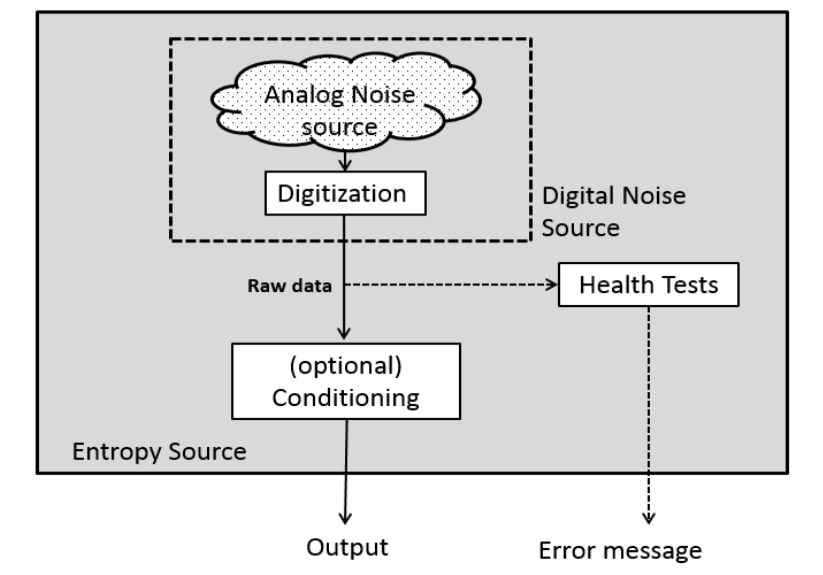
\includegraphics[width=0.75\textwidth]{figures/modle_zrodla.png}
      \caption{Model źródła entropii}
    \end{figure}

\stepcounter{footnote}\footnotetext[\value{footnote}]{\href{https://nvlpubs.nist.gov/nistpubs/SpecialPublications/NIST.SP.800-90B.pdf}{NIST SP 800-90B}}

\end{frame}
%---------------------------------------------------------
\begin{frame}
\frametitle{Wprowadzenie}


    \begin{figure}[H]
      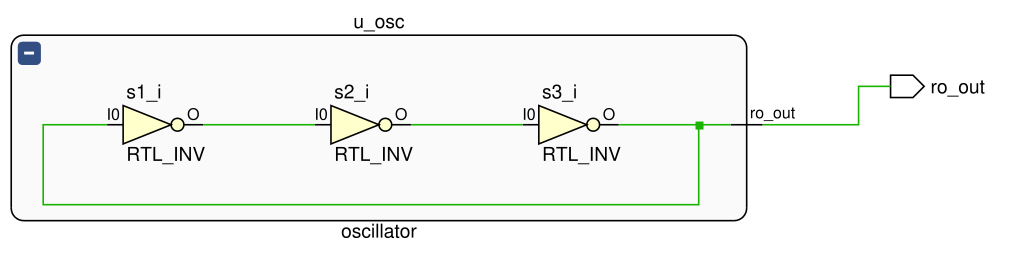
\includegraphics[width=\textwidth]{figures/oscylator.png}
      \caption{Prosty oscylator pierścieniowy}
    \end{figure}

\stepcounter{footnote}\footnotetext[\value{footnote}]{\href{https://nvlpubs.nist.gov/nistpubs/SpecialPublications/NIST.SP.800-90B.pdf}{NIST SP 800-90B}}

\end{frame}
%---------------------------------------------------------
\section{Testy bazowe}
%---------------------------------------------------------
\begin{frame}
\frametitle{Testy bazowe}

    \begin{figure}[H]
      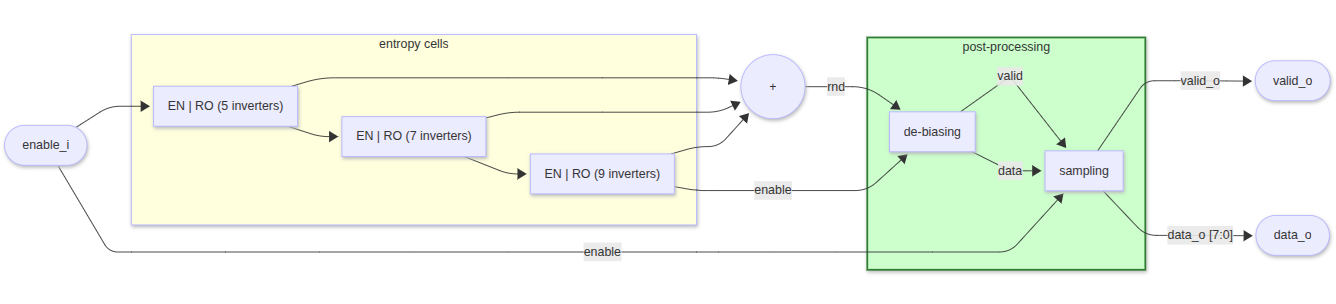
\includegraphics[width=\textwidth]{mermaid/png/2.png}
      \caption{Architektura modułu neoTRNG}
    \end{figure}

\end{frame}
%---------------------------------------------------------
\begin{frame}
\frametitle{4 przypadki bazowe}

\Large

\begin{center}
\begin{tabular}{ |c|c|c| } 
 \hline
  & de-biasing & sampling \\ 
 \hline
 RTL 1 & \colorbox{green}{TAK} & \colorbox{green}{TAK} \\ 
 \hline
 RTL 2 & \colorbox{green}{TAK} & \colorbox{red}{NIE} \\ 
 \hline
 RTL 3 & \colorbox{red}{NIE} & \colorbox{green}{TAK} \\
 \hline
 RTL 4 & \colorbox{red}{NIE} & \colorbox{red}{NIE} \\  
 \hline
\end{tabular}
\end{center}

\end{frame}
%---------------------------------------------------------
\begin{frame}
\frametitle{Porównanie zajętości}

\begin{center}
\begin{tabular}{ |c|c|c| } 
 \hline
  & LUT & FF \\ 
 \hline
 RTL 1 & ... & ... \\ 
 \hline
 RTL 2 & ... & ... \\ 
 \hline
 RTL 3 & ... & ... \\
 \hline
 RTL 4 & ... & ... \\  
 \hline
\end{tabular}
\end{center}

\end{frame}
%---------------------------------------------------------
\begin{frame}
\frametitle{Porównanie bitrate}

\begin{center}
\begin{tabular}{ |c|c| } 
 \hline
  & KiB/s \\ 
 \hline
 UART 921600bps & 90.5 \\ 
 \hline
 RTL 1 & 84 \\ 
 \hline
 RTL 2 & ... \\ 
 \hline
 RTL 3 & ... \\
 \hline
 RTL 4 & ... \\  
 \hline
\end{tabular}
\end{center}

\end{frame}
%---------------------------------------------------------
\begin{frame}[fragile]
\frametitle{ENT}

\begin{minted}[highlightlines={2, 5, 8, 11},linenos, breaklines]{bash}
~/tools/ent/src$ ./ent ch3_VN_CRC.bin 
Entropy = 7.999983 bits per byte.

~/tools/ent/src$ ./ent ch3_nVN_CRC.bin 
Entropy = 7.999981 bits per byte.

~/tools/ent/src$ ./ent ch3_VN_nCRC.bin 
Entropy = 7.893073 bits per byte.

~/tools/ent/src$ ./ent ch3_nVN_nCRC.bin 
Entropy = 7.341919 bits per byte.
\end{minted}
\end{frame}
%---------------------------------------------------------
\begin{frame}
\frametitle{NIST SP 800-22}


\begin{enumerate}
    \item finalAnalysisReport\_ch3\_VN\_CRC.txt
    \item finalAnalysisReport\_ch3\_nVN\_CRC.txt
    \item finalAnalysisReport\_ch3\_VN\_nCRC.txt
    \item finalAnalysisReport\_ch3\_nVN\_nCRC.txt
\end{enumerate}

\end{frame}
%---------------------------------------------------------
\begin{frame}[fragile]
\frametitle{NIST SP 800-90B}


\begin{minted}[highlightlines={2, 5, 8, 11}, linenos, breaklines, breakanywhere]{bash}
~/tools/SP800-90B_EntropyAssessment/cpp$ ./ea_non_iid ~/Desktop/magister/data/ch3_VN_CRC.bin 8
H_original: 7.487619

~/tools/SP800-90B_EntropyAssessment/cpp$ ./ea_non_iid ~/Desktop/magister/data/ch3_nVN_CRC.bin 8
H_original: 7.487620

~/tools/SP800-90B_EntropyAssessment/cpp$ ./ea_non_iid ~/Desktop/magister/data/ch3_VN_nCRC.bin 8
H_original: 6.738274

~/tools/SP800-90B_EntropyAssessment/cpp$ ./ea_non_iid ~/Desktop/magister/data/ch3_nVN_nCRC.bin 8
H_original: 5.623910
\end{minted}


\end{frame}
%---------------------------------------------------------
\section{Analiza rozmieszczenia}
%---------------------------------------------------------
\begin{frame}
\frametitle{Analiza rozmieszczenia}

    \begin{figure}[H]
      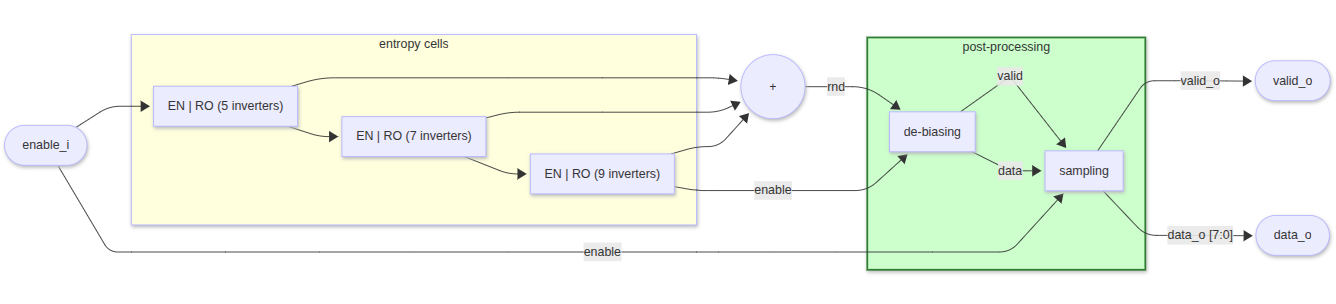
\includegraphics[width=\textwidth]{mermaid/png/2.png}
      \caption{Architektura modułu neoTRNG}
    \end{figure}


\Large

\textbf{Jak rozmieszczenie komórek entropii w fizycznym układzie (floorplan) wpłynie na entropię?}

\end{frame}
%---------------------------------------------------------
\section{Faza algorytmiczna i optymalizacja ekstrakcji}
%---------------------------------------------------------
\begin{frame}
\frametitle{Faza algorytmiczna i optymalizacja ekstrakcji}

\Large
\textbf{Porównanie innych metod post-processing'u}

\end{frame}
%---------------------------------------------------------
\section{Faza odporności i monitorowania online}
%---------------------------------------------------------
\begin{frame}
\frametitle{Faza odporności i monitorowania online}

\Large
\textbf{Rozszerzenie zakresu badań o zagadnienia związane z monitorowaniem 
działania źródła oraz wpływem warunków środowiskowych.}

\end{frame}
%---------------------------------------------------------
\section{NeoTRNG na FPGA dla RPI}
%---------------------------------------------------------
\begin{frame}
\frametitle{NeoTRNG na FPGA dla RPI}

\Large
\textbf{Dodatkowe aspekty implementacyjne oraz porównanie 
modułu wykorzystującego oscylatory pierścieniowe z komercyjnym generatorem Quantis.}

\end{frame}
%---------------------------------------------------------
\begin{frame}
\frametitle{}
\centering{\Huge{\textbf{Dziękuję za uwagę}}}
\end{frame}
%---------------------------------------------------------
\end{document}